% concatenated from GUSC_rings2.tex
\documentclass[12pt]{amsart}
\usepackage{amssymb}
\usepackage{amsmath, amscd}
\usepackage{amsthm}
\usepackage[table,xcdraw]{xcolor}
\usepackage{ulem}
\usepackage{tikz}
\usepackage{circuitikz}
\usetikzlibrary{positioning}
\usepackage[colorlinks=true, linkcolor=blue,urlcolor=blue]{hyperref}

\newtheorem{theorem}{Theorem}[section]
\newtheorem{mtheorem}[theorem]{Main Theorem}
\newtheorem{bbtheo}[theorem]{The Strong Black Box}
\newtheorem{observation}[theorem]{Observation}
\newtheorem{proposition}[theorem]{Proposition}
\newtheorem{lemma}[theorem]{Lemma}
\newtheorem{testlemma}[theorem]{Test Lemma}
\newtheorem{mlemma}[theorem]{Main Lemma}
\newtheorem{steplemma}[theorem]{Step Lemma}
\newtheorem{corollary}[theorem]{Corollary}
\theoremstyle{definition}
\newtheorem{notation}[theorem]{Notation}
\newtheorem{interconnection}[theorem]{Interconnection}
\newtheorem{example}[theorem]{Example}
\newtheorem{definition}[theorem]{Definition}
\newtheorem{exercise}[theorem]{Exercise}
\newtheorem{claim}[theorem]{Claim}

\newtheorem{conjecture}[theorem]{Conjecture}
\newtheorem{remark}[theorem]{Remark}
\newtheorem{note}[theorem]{Note}
\newtheorem{question}[theorem]{Question}
\newtheorem{problem}[theorem]{Problem}

\renewcommand{\labelenumi}{(\roman{enumi})}

%%%%%%%%%%%%%%%%%% page outfit %%%%%%%%%%%%%%%%%%%%%%%%%%%%%%%

\topmargin0cm \headheight0cm \headsep1cm \topskip0cm \textheight23cm \footskip1.8cm \textwidth15cm

\oddsidemargin0cm \evensidemargin0cm

\parindent15pt

\renewcommand{\baselinestretch}{1.0}

%%%%%%%%%%%%%%%%%%%% numbers %%%%%%%%%%%%%%%%%%

\newcommand{\N}{\mathbb{N}}
\newcommand{\Z}{\mathbb{Z}}
\newcommand{\Q}{\mathbb{Q}}
\newcommand{\re}{\mathbb{R}}
\newcommand{\co}{\mathbb{C}}
\newcommand{\p}{\mathbb{P}}
\newcommand{\U}{\mathcal{U}}
\newcommand{\V}{\mathcal{V}}
\newcommand{\Prop}{\mathbb{P}}
\newcommand{\B}{\mathcal{B}}
\newcommand{\A}{\mathcal{A}}
\newcommand{\qc}{\Z(p^\infty)}

\newcommand{\End}{{\rm End}}
\newcommand{\Aut}{{\rm Aut}}
\newcommand{\Hom}{{\rm Hom}}
\newcommand{\en}{endomorphism}
\newcommand{\ai}{anti--isomorphism}
\newcommand{\rk}{{\rm rk}}
\newcommand{\Ker}{{\rm Ker}}
\newcommand{\Ext}{{\rm Ext}}
\newcommand{\ent}{{\rm ent}}
\newcommand{\lcm}{{\rm lcm}}
\newcommand{\hcf}{{\rm hcf}}
\newcommand{\nbd}{{neighbourhood}}
\newcommand{\nbds}{{neighbourhoods}}
\newcommand{\topgp}{topological group}
\newcommand{\topsp}{topological space}
\newcommand{\hcd}{homogeneous completely decomposable}
\newcommand{\cd}{completely decomposable}
\newcommand{\hd}{homogeneous decomposable}
\newcommand{\dscy}{direct sum of cyclic}
\newcommand{\im}{{\rm Im}}
\newcommand{\w}{\omega}
\newcommand{\e}{\varepsilon}
\newcommand{\m}{\mu}
\newcommand{\n}{\nu}
\newcommand{\f}{\phi}
\newcommand{\hv}{\widehat\varphi}
\newcommand{\hF}{\widehat F}
\newcommand{\s}{\sigma}
\newcommand{\lo}{\lambda^{\aln}}
\newcommand{\al}{\aleph}
\newcommand{\ale}{\aleph_1}
\newcommand{\aln}{\aleph_0}
\newcommand{\cont}{2^{\aln}}
\newcommand{\xbar}{\bar x}
\newcommand{\ebar}{\bar }
\newcommand{\Gbar}{\bar G}
\newcommand{\Hbar}{\bar H}
\newcommand{\Abar}{\bar A}
\newcommand{\Ls}{\langle}
\newcommand{\Rs}{\rangle}
\newcommand{\oneonn}{\frac{1}{n}}
\newcommand{\oneonm}{\frac{1}{m}}
\newcommand{\oneonnm}{\frac{1}{nm}}
\newcommand{\monn}{\frac{m}{n}}
\newcommand{\dent}{\rm dent}
\newcommand{\dotT}{T^{\bullet}}
\newcommand{\la}{\langle}

\def\a{\alpha}
\def\b{\beta}
\def\g{\gamma}
\def\w{\omega}
\def\e{\varepsilon}
\def\o{\omega}
%\def\va{\varphi}
\def\k{\kappa}
\def\m{\mu}
\def\n{\nu}
\def\r{\rho}
\def\f{\phi}
\def\hv{\widehat\v}
\def\hF{\widehat F}
\def\v{\varphi}
\def\s{\sigma}
\def\l{\lambda}
\def\lo{\lambda^{\aln}}
\def\d{\delta}
%\def\z{\zeta}
\def\al{\aleph}
\def\ale{\aleph_1}
\def\aln{\aleph_0}
\def\cont{2^{\aln}}
\def\t{\tau}

\def\mra#1{\,\smash{\mathop{\rightarrow}\limits^{#1}}\,}
\def\mlra#1{\,\smash{\mathop{\longrightarrow}\limits^{#1}}\,}
\def\da{\downarrow}
\def\mda#1{\downarrow \rlap{$\vcenter{\hbox{$\scriptstyle#1$}}$}}
\def\lra{\longrightarrow}
\def\endo#1#2#3#4{\left[\begin{matrix}
                           #1 & #2 \cr
                           #3 & #4
                        \end{matrix}\right]}
\def\val#1{\vert #1 \vert}
\def\ov#1{\overline{#1}}
\def\bbvec#1{{\bf #1}}

%\usepackage[utf8]{inputenc}
%\usepackage{amssymb}
%\usepackage{amsmath, amscd}
%\usepackage{amsthm}
%\usepackage{xcolor}

%\topmargin0cm \headheight0cm \headsep1cm \topskip0cm \textheight21cm \footskip1.5cm \textwidth14cm
%\oddsidemargin0cm \evensidemargin0cm
%\parindent15pt

\topmargin0cm \headheight0cm \headsep1cm \topskip0cm \textheight23cm \footskip1.8cm \textwidth15cm

\oddsidemargin0cm \evensidemargin0cm

\parindent15pt

\renewcommand{\baselinestretch}{1.0}

\date\today

\begin{document}

\author[P. Danchev]{Peter Danchev}
\address{Institute of Mathematics and Informatics, Bulgarian Academy of Sciences, 1113 Sofia, Bulgaria}
\email{danchev@math.bas.bg; pvdanchev@yahoo.com}

\author[M. Esfandiar]{Mehrdad Esfandiar}
\address{Department of Mathematics and Computer Science Shahed University Tehran, Iran}
\email{mehrdad.esfandiar@shahed.ac.ir}	

\author[O. Hasanzadeh]{Omid Hasanzadeh}
\address{Department of Mathematics, Tarbiat Modares University, 14115-111 Tehran Jalal AleAhmad Nasr, Iran}
\email{o.hasanzade@modares.ac.ir; hasanzadeomiid@gmail.com}

\title[Rings whose non-units elements are uniquely strongly clean]{\small Rings whose non-invertible elements are \\ uniquely strongly clean}
\keywords{unit, clean element (ring), uniquely clean element (ring), strongly clean element (ring), uniquely strongly clean element (ring)}
\subjclass[2010]{16S34, 16U60}

\maketitle

\begin{abstract}
We define and investigate in details the class of so-termed {\it GUSC} rings, that are those rings whose non-invertible elements are uniquely strongly clean. These rings are a common non-trivial generalization of the so-called {\it USC} rings, introduced by Chen-Wang-Zhou in J. Pure \& Appl. Algebra (2009), which are rings whose elements are uniquely strongly clean. These rings also properly generalize the so-named {\it GUC} rings, defined by Guo-Jiang in Bull. Transilvania Univ. Bra\c{s}ov (2023), which are rings whose non-invertible elements are uniquely clean.
\end{abstract}

\section{Introduction and Basic Concepts}

Everywhere in the present paper, let $R$ be an associative but {\it not} necessarily commutative ring having identity element, usually stated as $1$. Standardly, for such a ring $R$, the letters $U(R)$, $Nil(R)$ and $Id(R)$ are designed for the set of invertible elements (also termed as the unit group of $R$), the set of nilpotent elements and the set of idempotent elements in $R$, respectively. Likewise, $J(R)$ denotes the Jacobson radical of $R$, and $Z(R)$ denotes the center of $R$. We also write $ucn(R)$ for the set of all uniquely clean elements of $R$ as well as the ring of $n\times n$ matrices over $R$ and the ring of $n\times n$ upper triangular matrices over $R$ are denoted by $M_{n}(R)$ and $T_{n}(R)$, respectively.

Traditionally, a ring is said to be {\it abelian} if each of its idempotents is central, that is, $Id(R)\subset Z(R)$. For all other unexplained explicitly notions and notations, we refer to the classical source \cite{61} or to the cited in the bibliography research sources. For instance, consulting with \cite[Definition 3.4]{5}, we set $$ucn_{0}(R):=\{ e+j:e^{2}=e\in Z(R), j\in J(R)\}.$$

In order to share our achievements here, we now need the necessary background material as follows: Mimicking \cite{8}, an element $a$ from a ring $R$ is called {\it clean} if there exists $e\in Id(R)$ such that $a-e\in U(R)$. Then, $R$ is said to be {\it clean} if each element of $R$ is clean. In addition, $a$ is called {\it strongly clean} provided $ae=ea$ and, if each element of $R$ are strongly clean, then $R$ is said to {\it strongly clean} too.
On the other hand, imitating \cite{3}, $a\in R$ is called {\it uniquely clean} if there exists a unique $e \in Id(R)$ such that $a-e \in U(R)$. In particular, a ring $R$ is said to be {\it uniquely clean} (or, shortly, just {\it UC}) if every element in $R$ is uniquely clean.

Generalizing these concepts, in \cite{2} was defined an element $a \in R$ to be {\it uniquely strongly clean} if there exists a unique $e \in Id(R)$ such that $a-e \in U(R)$ and $ae=ea$. In particular, a ring $R$ is {\it uniquely strongly clean} (or, shortly, just {\it USC}) if each element in $R$ is uniquely strongly clean.

Continuing in a similar vein this terminology, expanding the first part of the presented above notions, in \cite{1} a ring is called a {\it generalized uniquely clean} ring (or just {\it GUC} for short) if any non-invertible element is uniquely clean.

\medskip

Our work in this article targets to extend considerably the last definition by defining and exploring the following key instrument: A ring is called a {\it generalized uniquely strongly clean} ring (or just {\it GUSC} for short) if every non-invertible element is uniquely strongly clean.

The relationships between all of these ring classes are visualized via the next diagram:

\bigskip

\begin{center}
	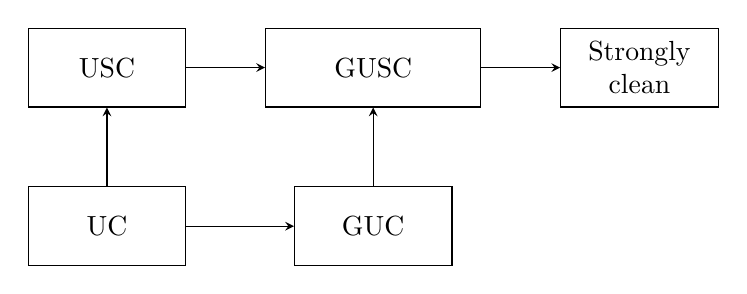
\begin{tikzpicture}
		\node[draw, minimum width=2cm, minimum height=1cm, text width=1.75cm, align=center]  (a) {USC};
		\node[draw, minimum width=2cm, minimum height=1cm, text width=2.5cm, align=center, right=of a](b){GUSC};
		\node[draw, minimum width=2cm, minimum height=1cm, text width=1.75cm, align=center, below=of b](c){GUC};
		\node[draw, minimum width=2cm, minimum height=1cm, text width=1.75cm, align=center, right=of b](d){Strongly clean};
		\node[draw, minimum width=2cm, minimum height=1cm, text width=1.75cm, align=center, below=of a](f){UC};
		\draw[-stealth] (a) -- (b);
		\draw[-stealth] (c) -- (b);
		\draw[-stealth] (f) -- (a);
		\draw[-stealth] (f) -- (c);
		\draw[-stealth] (b) -- (d);
	\end{tikzpicture}
\end{center}

\bigskip

Our motivating tool here is to develop a substantial study on this {\bf new} class of rings showing that their complete classification is extremely difficult and rather complicated.

\section{Examples and Main Results}

We begin our considerations by marking the following four simple but useful observations.

\begin{example}\label{exam1.7}
\begin{enumerate}
\item
Any UC ring is USC, but the converse is {\it not} true in general. In fact, the ring $T_{2}(\mathbb{Z}_{2})$ is USC that is {\it not} UC.

\item
Any UC ring is GUC, but the converse is {\it not} true in general. Indeed, the ring $\mathbb{Z}_{5}$ is GUC that is {\it not} UC.

\item
Any USC ring is GUSC, but the converse is {\it not} true in general. In fact, the ring $\mathbb{Z}_{(3)}=\left\{ \dfrac{a}{b} ~ \Big| ~ a,b \in \mathbb{Z}, (3,b)=1\right\}$ is GUSC that is {\it not} USC.

\item
Any GUC ring is GUSC, but the converse is {\it not} true in general. Indeed, the ring $M_{2}(\mathbb{Z}_{2})$ is GUSC that is {\it not} GUC.

\item
Any GUSC ring is strongly clean, but the converse is {\it not} true in general. To demonstrate that, for an arbitrary prime number $p$, let $\hat{\mathbb{Z}_{p}}$ be the ring of $p$-adic integers. In view of \cite[Theorem 2.4]{10}, the ring $M_{2}(\hat{\mathbb{Z}}_{p})$ is strongly clean which is manifestly {\it not} USC in virtue of \cite[Corollary 7]{2}. Also, a plain check shows that it is too {\it not} GUSC.
\end{enumerate}
\end{example}

We, furthermore, continue with a series of helpful technicalities.

\begin{lemma}\label{lem2.1}
An element $a$ in a ring $R$ is USC if, and only if, so is $1-a$ in $R$.
\end{lemma}

\begin{proof} Straightforward.
\end{proof}

\begin{lemma}\label{lem2.2}
If $R$ is a GUSC ring, then $R$ is strongly clean.
\end{lemma}

\begin{proof}
Choosing $a \in R$, so $a \in U(R)$ or $a \not\in U(R)$. If $a \in U(R)$, then $a$ is known to be a strongly clean element. If, however, $a\not\in U(R)$, then by assumption $a$ is USC element, and thus $a$ is a strongly clean element. Finally, in both cases, $R$ is strongly clean, as expected.
\end{proof}

\begin{lemma}\label{lemma 2.6}
Let $R$ be a GUSC ring with $2 \in U(R)$ and, for every $u \in U(R)$, we have $u^2 = 1$. Then, $R$ is a commutative ring.
\end{lemma}

\begin{proof}
Firstly, we show that \( R \) is reduced, i.e., \( R \) contains no non-trivial nilpotent elements, so suppose \( q \in Nil(R) \). Then, \( (1 \pm q) \in U(R) \), whence
\[ 1 - 2q + q^2 = (1-q)^2 = 1 = (1+q)^2 = 1 + 2q + q^2. \]
Thus, \( 4q = 0 \). Since \( 2 \in U(R) \), we conclude \( q = 0 \). Hence, \( R \) is reduced and, consequently, \( R \) is abelian.
	
Moreover, for any \( u, v \in U(R) \), we have \( u^2 = v^2 = (uv)^2 = 1 \). Therefore, \( uv = (uv)^{-1} = v^{-1} u^{-1} = vu \), and hence the units commute with each other.
	
In addition, let \( x, y \in R \). We consider the following four possible cases:
	
1. \( x, y \in U(R) \): since the units commute, it must be that \( xy = yx \).
	
2. \( x, y \notin U(R) \): since \( R \) is a GUSC ring, there exist \( e, f \in Id(R) \) and $u, v\in U(R)$ such that \( x = e+u \) and \( y = f+v \). So, \( xy = yx \), because \( R \) is abelian and the units commute.
	
3. \( x \in U(R) \) and \( y \notin U(R) \): in this case, there exist \( e \in Id(R) \) and $u\in U(R)$ such that \( y = e+u \). Then, $xy=x(e+u)=xe+xu$. But, we have $xy=ex+ux=(e+u)x=yx$, because $R$ is abelian and the units commute.
	
4. \( x \notin U(R) \) and \( y \in U(R) \): similarly to case (3), we can easily see that \( xy = yx \).	

This completes our arguments after all.
\end{proof}

\begin{lemma}\label{lem2.3}
If $\displaystyle\prod_{i \in I} R_i$ is GUSC, then each direct component $R_i$ is GUSC too.
\end{lemma}

\begin{proof}
Choose an arbitrary $a_{i}\in R_{i}$, where $a_{i}\not\in U(R_{i})$, whence $$(1,1,\ldots , a_{i}, 1, \ldots )\not\in U(\prod R_{i}).$$ Thus, $(1,1,\ldots ,a_{i},1,\ldots )$ is USC and hence $a_{i}$ is USC, as required.

If, however, some element $a_{i}$ is not USC, then we have two different strongly clean decompositions for $a_{i}$ and so we have two different strongly clean decompositions for $(1,1,\ldots ,a_{i},1,\ldots )$. This shows the desired contradiction, as needed.
\end{proof}

We note that the opposite of Lemma \ref{lem2.3} is manifestly false. To exhibit that, both $\mathbb{Z}_{2}$ and $\mathbb{Z}_{3}$ are GUSC. But, the direct product $\mathbb{Z}_2 \times \mathbb{Z}_3$ is {\it not} GUSC, because the element $(0,2)$ is obviously {\it not} invertible in $\mathbb{Z}_2 \times \mathbb{Z}_3$ and $(0,2)=(1,0)+(1,2)=(1,1)+(1,1)$ are two different strongly clean decompositions of $(0,2)$ in $\mathbb{Z}_2 \times \mathbb{Z}_3$, so that $(0,2)$ is really {\it not} USC element, as pursued.

\begin{proposition}\label{prop2.5}
The direct product $\displaystyle\prod_{i\in I} R_i$ ($|I| \geq 2$) is GUSC if, and only if, each $R_i$ is USC.
\end{proposition}

\begin{proof}
Letting each $R_{i}$ be USC, then $\prod R_{i}$ is USC employing \cite[Example 2]{2} and hence $\prod R_{i}$ is trivially GUSC.

Conversely, assume that $\prod R_{i}$ is GUSC and that $R_{j}$ is {\it not} USC for some index $j\in I$. Then, there exists $a\in R_{j}$ which is {\it not} USC. Hence, $(0,\ldots ,0,a,0,\ldots )$ is {\it not} USC in $\prod R_{i}$. However, it is readily seen that $(0,\ldots ,0,a,0,\ldots )$ is {\it not} invertible in $\prod R_{i}$ and thus, by hypothesis, $(0,\ldots ,0,a,0,\ldots )$ is {\it not} USC -- an absurd. Therefore, every $R_{i}$ is USC, as wanted.
\end{proof}

Three consequences validate now.

\begin{corollary}
Let $L=\prod_{i \in I} R_i$ with $|I| \geq 2$ be the direct product of rings $R_i \cong R$. Then, $L$ is a GUSC ring if, and only if, $L$ is a USC ring if, and only if, $R$ is USC.
\end{corollary}

\begin{corollary}
For any $n \geq 2$, the ring $R^n$ is GUSC if, and only if, $R^n$ is USC if, and only if, $R$ is USC.
\end{corollary}

\begin{corollary}\label{cor2.6}
Let $R$ be a ring and $0\neq e \in Id(R)\cap Z(R)$. If $R$ is GUSC, then so is $eRe$. In addition, if $e$ is non-trivial, i.e., $e\not= 0,1$, then $eRe$ is USC.
\end{corollary}

\begin{proof}
Assume $R$ is GUSC. We have decomposed $$R=eRe \oplus (1-e)R(1-e).$$ Hence, $eRe$ is GUSC applying Lemma \ref{lem2.3}. If $e$ is {\it not} trivial, then $eRe$ is USC utilizing Proposition \ref{prop2.5}, as claimed.
\end{proof}

We next proceed by proving the following slight refinement of the last corollary.

\begin{proposition}\label{1}
Let $R$ be a ring and $0\neq e \in Id(R)$. If $R$ is GUSC, then so is $eRe$.
\end{proposition}

\begin{proof}
Suppose $R$ is a GUSC ring, so it is strongly clean in view of Lemma~\ref{lem2.2} and hence $eRe$ is strongly clean viewing \cite[Theorem 1.1.12]{13}.

Now, choose $a \in eRe$ to be not invertible in $eRe$. Write $$a=e_{1}+u_{1}=e_{2}+u_{2},$$ where $e_{1}$, $e_{2}$ are idempotents in $eRe$ and $u_{1}$, $u_{2}$ are units in $eRe$. Thus, $v_{i}=u_{i}+(1-e)$ are units in $R$ for $i=1,2$. So, $e_{1}+v_{1}=e_{2}+v_{2}$ are two strongly clean decompositions in $R$. However, as $a$ is chosen to be non-invertible in $eRe$, it must be that $e_{i}+v_{i}$ is not invertible in $R$ for $i=1,2$. Then, by hypothesis, we deduce $e_{1}=e_{2}$. Hence, $eRe$ is GUSC, as asserted.  	
\end{proof}	

Before continuing further, a useful example to know is the following one.

\begin{example}\label{exam2.7}
If $R$ is a local ring, then $R$ is GUSC.
\end{example}

\begin{proof}
Let $a \in R\setminus U(R)$. So, one inspects that $a=1+(a-1)$ is the only strongly clean decomposition for $a$, and thus $a$ is GUSC, as requested.
\end{proof}

However, the converse of the Example~\ref{exam2.7} is false. For instance, it is quite clear that $T_{2}(\mathbb{Z}_{2})$ is GUSC, but is obviously {\it not} local.

\medskip

We remember that a ring $R$ is called {\it semi-potent} if every one-sided ideal {\it not} contained in $J(R)$ contains a non-zero idempotent. In addition, a semi-potent ring $R$ is called {\it potent} if all idempotents of $R$ lift modulo $J(R)$. Semi-potent rings and potent rings were also named as {\it $I_{0}$-rings} and {\it $I$-rings}, respectively, by Nicholson in \cite{11}. Recall, moreover, that in \cite{55} a ring $R$ is called {\it exchange}, provided that, for any $a$ in $R$, there is an idempotent $e\in R$ such that $e\in aR$ and $e\in (1-a)R$ (compare with \cite{3} as well).

\begin{proposition}\label{prop2.8}
Let $R$ be a ring and $Id(R)=\{0,1\}$. Then, the following items are equivalent:
\begin{enumerate}
\item
$R$ is a local ring.
\item
$R$ is a GUSC ring.
\item
$R$ is a strongly clean ring.
\item
$R$ is a clean ring.
\item
$R$ is an exchange ring.
\item
$R$ is a potent ring.
\item
$R$ is a semi-potent.
\item
$R$ is a GUC ring.
\end{enumerate}
\end{proposition}

\begin{proof}
(i) $\Rightarrow$ (ii). It is quite elementary owing to Example \ref{exam2.7}.\\
(ii) $\Rightarrow$ (iii). It is pretty easy according to Lemma \ref{lem2.2}.\\
(iii) $\Rightarrow$ (vi) $\Rightarrow$ (v) $\Rightarrow$ (vi) $\Rightarrow$ (vii) $\Rightarrow$ (i). All evident.\\
(i) $\Rightarrow$ (viii). It is apparent that an analogous proof to that of Example \ref{exam2.7} works.\\
(viii) $\Rightarrow$ (i). Let $a\in R$ with $a\not\in U(R)$. It is now sufficient to prove that $a-1\in U(R)$. To this goal, by hypothesis, $a$ is uniquely clean, so we have $a=e+u$, where $e\in {Id}(R)=\{0,1\}$ and $u\in U(R)$. If $e=0$, it must be that $a=u\in U(R)$, a contradiction. If $e=1$, we infer $a=1+u$ and hence $a-1=u\in U(R)$, as desired.
\end{proof}

The next necessary and sufficient condition somewhat completely characterizes GUC rings in terms of GUSC rings.

\begin{proposition}\label{prop2.9}
A ring $R$ is GUC if, and only if, $R$ is GUSC and abelian.
\end{proposition}

\begin{proof}
Suppose foremost that $R$ is GUSC and abelian. So, one observes that $R$ is either local or USC. If $R$ is local, then $R$ is UC in accordance with \cite[Example 2.8]{1} whence it is GUC.

If, however, $R$ is USC, then $R$ is UC thanks to \cite[Example 4]{2} and hence $R$ is GUC. Consequently, in both cases, $R$ is GUC.

The other implication is straightforward.
\end{proof}

Our presentation in what follows unambiguously illustrates that the complete characterization of non-abelian GUSC rings is insurmountable at this stage, so we perceive in the sequel only partial descriptions of these rings.

\medskip

The following crucial observation seems {\it not} to appear in \cite{1}.

\begin{proposition}\label{pro2.2}
In any ring, idempotents and nilpotent elements are USC elements.
\end{proposition}

\begin{proof}
Let $e$ be an arbitrary idempotent element in a ring $R$. Then, we have that $e=(1-e)+(2e-1)$ is a strongly clean decomposition for $e$. Now, suppose that $e=f+u$ another strongly clean decomposition for $e$. It suffices to show only that $f=1-e$. In fact, we know that $(e-f)^2\in Id(R)\cap U(R)$ and hence $(e-f)^2=1$. So, $f=(2f-1)e+1$. Therefore, $$f=(2f-1)f=(2f-1)((2f-1)e+1)=(2f-1)(2f-1)e+(2f-1)=e+2f-1,$$ whence, $f=1-e$, as sufficed.

Suppose now that $q\in Nil(R)$ is chosen arbitrarily. Then, we have that $q=1+(q-1)$ is a strongly clean decomposition for $q$. Letting $q=e+u$ be an another strongly clean decomposition, it needs to show only that $e=1$. In fact, assume that $q^n=0$ for some natural $n>1$, and so $(e+u)^n=0$. Since $eu=ue$, one checks that $u^n\in eR$. That is why, $e=1$, as needed.
\end{proof}

Our pivotal demonstration is this one (compare with Example~\ref{exam1.7}(iv) too).

\begin{example}\label{exmnew}
The ring $M_2(\mathbb{Z}_2)$ is a GUSC ring, however is {\it not} a USC ring. This enables us that, under some extra conditions, matrix rings can be GUSC rings, but one knows that matrix rings are {\it never} USC rings.

Indeed, it follows from the equality $$M_2(\mathbb{Z}_2) = U(M_2(\mathbb{Z}_2)) \cup Id(M_2(\mathbb{Z}_2)) \cup Nil(M_2(\mathbb{Z}_2))$$ combined with Proposition~\ref{pro2.2} that $M_2(\mathbb{Z}_2)$ is GUSC, as asked.
\end{example}

With these arguments at hand, one can extract the following interesting affirmation.

\begin{corollary}\label{cor2.11}
For each $k \in \mathbb{N}$, the ring $M_2(\mathbb{Z}_{2^k})$ is GUSC.
\end{corollary}

We now come to our first major statement which sounds a bit curiously.

\begin{theorem}\label{3}
For any ring $S \neq 0$ and any integer $n \ge 3$, the ring $M_n(S)$ need not be GUSC.
\end{theorem}

\begin{proof}
Since it is well known that $M_3(S)$ is isomorphic to a corner subring of $M_n(S)$, we need to establish that $M_3(S)$ is {\it not} a GUSC ring invoking Proposition~\ref{1}. To this purpose, consider the matrix
$$A =\begin{pmatrix}
		1 & 1 & 0 \\
		1 & 0 & 0 \\
		0 & 0 & 0
\end{pmatrix} \notin U(M_3(S)).$$ A plain inspection gives us that $A$ is {\it not} a strongly clean element and hence it is not a uniquely strongly clean element, as promised. Therefore, $R$ cannot be a GUSC ring, as aimed.
\end{proof}

The next construction is worthy of recording.     	

\begin{example}\label{exam2.13}
Let $R$ be a ring. If $T_{n}(R)$ is a GUSC ring, then $R$ is also GUSC. The converse holds, provided $R$ is commutative and USC (or just UC).
\end{example}

\begin{proof}
Let $T_{n}(R)$ be GUSC and put $e:={\rm diag}(1,0,\ldots ,0)\in T_{n}(R)$. Then, one sees that $R\cong eT_{n}(R)e$, so that $R$ is a GUSC ring using Proposition \ref{1}.

The reciprocal claim is clear exploiting \cite[Theorem 10]{2}.
\end{proof}

We continue our work with the following assertions, the first of which is immediate but worthy of mentioning.

\begin{proposition}\label{prop2.14}
For any ring $R$, the polynomial ring $R[x]$ is not GUSC.
\end{proposition}

\begin{proof}
We know that $R[x]$ is not clean, so it is {\it not} strongly clean and thus is definitely {\it not} GUSC.
\end{proof}

The next claim surprisingly does {\it not} appear in \cite{1}.

\begin{lemma}\label{lem2.18}
If $R$ is a USC ring, then $ucn(R)=ucn_0(R)$.
\end{lemma}

\begin{proof}
For any ring $R$, we know that $$ucn_0(R)=\left\{e+j \mid e^2=e \in Z(R), j \in J(R)\right\}.$$ We are also aware that $R$ is a clean ring, and thus idempotents lift modulo $J(R)$. Moreover, the quotient $\dfrac{R}{J(R)}$ is boolean bearing in mind \cite[Corollary 18]{2}, so that the equality $$ucn\left(\dfrac{R}{J(R)}\right)=ucn_0\left(\dfrac{R}{J(R)}\right)$$ forces $ucn(R)=ucn_{0}(R)$ knowing \cite[Proposition 3.6]{1}, as stated.
\end{proof}

We are now ready to attack and resolve in the affirmative \cite[Question 4.8]{1} asking: Is it true that $R$ is a GUC ring if, for every non-invertible element $a\in R$, there exists an unique idempotent $e\in R$ such that $a-e\in J(R)$?

\begin{proposition}\label{prop2.21}
The answer to this question is positive.
\end{proposition}

\begin{proof}
First, we menage to show that $Nil(R)\subseteq J(R)$. In fact, let $a\in Nil(R)$.

If, for a moment, $a\in U(R)$, then $a=0$ and hence $a\in J(R)$.

If, however, $a\not\in U(R)$, there will exist an unique idempotent $e\in R$ such that $a-e\in J(R)$. Then, we have $a+J(R)=e+J(R)$, and thus $$a+J(R)\in Id(\dfrac{R}{J(R)}) ~ \bigvee ~ a+J(R)\in Nil(\dfrac{R}{J(R)}).$$ So, it must be that $a+J(R)=J(R)$ whence $a\in J(R)$.

Now, we intend to prove that, for every non-invertible element $a\in R$, there exists an unique central idempotent $e\in R$ such that $a-e\in J(R)$. In fact, let $a\in R$, where $a\not\in U(R)$, so by hypothesis there is an unique idempotent $e\in R$ such that $a-e\in J(R)$. It now suffices to establish that $e\in Z(R)$. To this aim, for each $r\in R$, $$er(1-e), (1-e)re\in Nil(R)\subseteq J(R)$$ and $$e+(1-e)re, e+er(1-e)\in Id(R),$$ so we deduce $$a-(e+er(1-e)),a-(e+(1-e)re)\in J(R).$$ However, by the uniqueness, we derive $$e+(1-e)re=e+er(1-e)=e.$$ Therefore, $er=ere=re$ and hence $e\in Z(R)$, as we want. Finally, working with \cite[Theorem 3.5]{1}, we can conclude that $R$ is GUC, as we promised above.
\end{proof}

Let $R$ be a ring and $M$ a bi-module over $R$. The trivial extension of $R$ and $M$ is defined as
\[ T(R, M) = \{(r, m) : r \in R \vee m \in M\}, \]
with addition defined component-wise and multiplication defined by
\[ (r, m)(s, n) = (rs, rn + ms). \]
The trivial extension $T(R, M)$ is isomorphic to the subring consisting of matrices of the sort
\[ \left\{ \begin{pmatrix} r & m \\ 0 & r \end{pmatrix} : r \in R \text{ and } m \in M \right\} \]
of the formal $2 \times 2$ matrix ring $\begin{pmatrix} R & M \\ 0 & R \end{pmatrix}$, and likewise additionally $T(R, R) \cong R[x]/\left\langle x^2 \right\rangle$.

We, moreover, note that the set of units of the trivial extension $T(R, M)$ is precisely
\[ U(T(R, M)) = T(U(R), M). \]

\noindent The next statement is worthwhile.

\begin{proposition}\label{prop2.22}
If the trivial extension $T(R,M)$ is a GUSC ring, then $R$ is a GUSC ring. The converse implication holds, provided $em=me$ for all $m\in M$ and $e\in Id(R)$.
\end{proposition}

\begin{proof}
First we claim that, if $(e,m)^{2}=(e,m)\in T(R,M)$, then $e^{2}=e$ and $m=0$. In fact, the equality $(e,m)^{2}=(e,m)$ automatically gives by comparison that $e^{2}=e$ and $em+me=m$. So, by hypothesis, we have $2em=m$, whence $2em=em$ and so $em=0$. Thus, $2em=0$ and hence $m=0$, proving the claim.
	
Choose now $a\in R$, where $a\not\in U(R)$, so that $(a,0)\notin U(T(R,M))$ and thus $(a,0)$ is a USC element in $T(R,M)$. Then, $a$ is a USC element in $R$, because for otherwise, if $a$ has two different strongly clean decompositions, then $(a,0)$ has two different strongly clean decompositions contradicting our assumption.

For the reciprocal implication, choose $(a,m)\in T(R,M)$, where $(a,m)\notin U(T(R,M))$, so that $a\not\in U(R)$ as for otherwise, if $a\in U(R)$, then $(a,m)\in U(T(R,M))$ with inverse $(a^{-1},-a^{-1}ma^{-1})$, a contradiction, and therefore by hypothesis $a$ is a USC element. Consequently, the element $(a,m)$ is USC, because for otherwise, if $(a,m)=(e,0)+(u,m)=(f,0)+(v,m)$, where $(e,0), (f,0)\in Id(T(R,M))$, $(u,m),(v,m)\in U(T(R,M))$ and
$(e,0)(u,m)=(u,m)(e,0)$, $(f,0)(v,m)=(v,m)(f,0)$, then we will have $$a=e+u=f+v,$$ where $e,f\in Id(R)$, $u,v\in U(R)$ and $eu=ue$, $fv=vf$. Finally, $a$ possesses two strongly clean decompositions which is impossible.
\end{proof}

Two direct consequences sound as follows.

\begin{corollary}
If the trivial extension $T(R,R)$ is a GUSC ring, then $R$ is a GUSC ring. The opposite assertion holds when the ring $R$ is abelian.
\end{corollary}

\begin{corollary}
Let $R$ be an abelian ring, and let $M$ be a bi-module over $R$. Then, the following four statements are equivalent:
\begin{enumerate}
\item
$R$ is a GUSC ring.
\item
$T(R, R)$ is a GUSC ring.
\item
$R[x]/\left\langle x^2 \right\rangle$ is a GUSC ring.
\item
$R[[x]]/\langle x^2\rangle$ is a GUSC ring.
\end{enumerate}
\end{corollary}

Consider now $R$ to be a ring and $M$ to be a bi-module over $R$. Set $$BT(R,M) := \{ (a, m, b, n) | a, b \in R, m, n \in M \}$$ with addition defined component-wise and multiplication defined by $$(a_1, m_1, b_1, n_1)(a_2, m_2, b_2, n_2) = (a_1a_2, a_1m_2 + m_1a_2, a_1b_2 + b_1a_2, a_1n_2 + m_1b_2 + b_1m_2 +n_1a_2).$$ Then, $BT(R,M)$ becomes a ring which is isomorphic to $T(T(R, M), T(R, M))$. We also have the equality $$BT(R, M) =
\left\{\begin{pmatrix}
	a &m &b &n\\
	0 &a &0 &b\\
	0 &0 &a &m\\
	0 &0 &0 &a
\end{pmatrix} |  a,b \in R, m,n \in M\right\}.$$ In particular, we obtain the following isomorphism as rings: $$\dfrac{R[x, y]}{\langle x^2, y^2\rangle} \rightarrow BT(R, R)$$ via the map $$a + bx + cy + dxy \mapsto
\begin{pmatrix}
	a &b &c &d\\
	0 &a &0 &c\\
	0 &0 &a &b\\
	0 &0 &0 &a
\end{pmatrix}.$$

We, thereby, arrive at the following three corollaries.

\begin{corollary}
If $BT(R,M)$ is a GUSC ring, then $R$ is a GUSC ring. The converse is true, provided $em=me$ for all $m\in M$ and $e\in Id(R)$.
\end{corollary}

\begin{corollary}
If $BT(R,R)$ is a GUSC ring, then $R$ is a GUSC ring. The converse is valid when the ring $R$ is abelian.
\end{corollary}

\begin{corollary}
Let $R$ be an abelian ring, and let $M$ be a bi-module over $R$. Then, the following three statements are equivalent:
\begin{enumerate}
\item
$R$ is a GUSC ring.
\item
$BT(R, R)$ is a GUSC ring.
\item
$R[x, y]/\langle x^2, y^2\rangle$ is a GUSC ring.
\end{enumerate}
\end{corollary}

Let $R$ be a ring, and let $M$ be a bi-module over $R$ that is a non-unital ring in which the equalities $(mn)r=m(nr)$, $(mr)n=m(rn)$ and $(rm)n=r(mn)$ are fulfilled for all $m,n\in M$ and $r\in R$. Then, the ideal-extension $I(R,M)$ of $R$ by $M$ is defined as the additive abelian group $I(R,M)=R\oplus M$ with multiplication given by $$(r,m)(s,n)=(rs, rn+ms+mn).$$

\medskip

We are now in a position to establish the validity of the following statement.

\begin{proposition}\label{prop2.23}
If the ideal extension $I(R,M)$ is a GUSC ring, then $R$ is a GUSC ring. The converse holds provided the following conditions are satisfied:
\begin{enumerate}
\item[(a)]
If $e\in Id(R)$, then $em=me$ for all $m\in M$.
\item[(b)]
If $m\in M$, then $m+n+mn=0$ for some $n\in M$.
\end{enumerate}
\end{proposition}

\begin{proof}
The necessity is rather identical to the arguments given in Proposition \ref{prop2.22}.

To prove the sufficiency, we first know with the help of (a), (b) and \cite[Proposition7]{3} that each idempotent of $I(R,M)$ is of the type $(e,0)$, where $e^{2}=e$, as well as that each unit of $I(R,M)$ is of the type $(u,m)$, where $u\in U(R)$, $m\in M$.

Now, choosing $(a,m)\in I(R,M)$, where $(a,m)\not\in U(I(R,M))$, we observe that $a\not\in U(R)$. Thus, by hypothesis, the element $a$ is USC, and so $(a,m)$ is a USC element in $I(R,M)$, because for otherwise, if $(a,m)$ has two different strongly clean decompositions, then arguing as in the proof of Proposition \ref{prop2.22}, the element $a$ has two different strongly clean decompositions which is false. The assertion sustained.
\end{proof}

\begin{proposition}\label{2}
Let $R$ be a GUSC ring. Then, for any $n>2$, there does not exist $0\neq e\in Id(R)$ such that $eRe\cong M_{n}(S)$ for some ring $S$.
\end{proposition}

\begin{proof}
Let us assume the contrary, namely that there exists $0\neq e\in Id(R)$ such that $eRe\cong M_{n}(S)$ for some ring $S$. But, since by assumption $R$ is GUSC, it follows from Proposition \ref{1} that the corner subring $eRe$ is GUSC too, and hence $M_{n}(S)$ is GUSC as well. This, however, contradicts Theorem \ref{3}, sustaining our statement.
\end{proof}

Recall that a set $\{e_{ij} : 1 \le i, j \le n\}$ of non-zero elements of $R$ is said to be a {\it system of $n^2$ matrix units}, provided that $e_{ij}e_{st} = \delta_{js}e_{it}$, where $\delta_{jj} = 1$ and $\delta_{js} = 0$ for $j \neq s$. In this case, $e := \sum_{i=1}^{n} e_{ii}$ is an idempotent of $R$ and $eRe \cong M_n(S)$, where $$S = \{r \in eRe : re_{ij} = e_{ij}r, \text{for all} i, j = 1, 2, . . . , n\}.$$
Remember also that a ring $R$ is said to be {\it Dedekind-finite} if $ab=1$ insures $ba=1$ for any $a,b\in R$. In other words, all one-sided units in the ring are two-sided.

\medskip

What we can said now is the following observation.

\begin{proposition}\label{pro3.32}
Every GUSC ring is Dedekind-finite.
\end{proposition}

\begin{proof}
Suppose $R$ is a GUSC ring. If we assume the contrary, namely that $R$ is not a Dedekind-finite ring, then there exist two elements $a, b \in R$ such that $ab = 1$ but $ba \neq 1$. Setting $e_{ij} := a^i(1-ba)b^j$ and
$e :=\sum_{i=1}^{n}e_{ii}$, a routine verification guarantees that there exists a non-zero ring $S$ such that $eRe \cong M_n(S)$. However, Proposition \ref{1} informs us that the corner $eRe$ is a GUSC ring, so that $M_n(S)$ has also be a GUSC ring, contradicting Theorem \ref{3}. This substantiates our claim.
\end{proof}	

%\begin{remark} For $e_{11}$, we have $$e_{11}=a(1-ba)b=ab-(ab)(ab)=0.$$ In the same way, $e_{kk}=0$ for all $k\in \mathbb{N}$. Hence, $eRe=\{0\}$, as required.
%\end{remark}

Let $Nil_{*}(R)$ denote the {\it prime radical} (or, in other words, the {\it lower nil-radical}) of a ring $R$, i.e., the intersection of all prime ideals of $R$. We know that $Nil_{*}(R)$ is a nil-ideal of $R$.

Besides, it is also long known that a ring $R$ is {\it $2$-primal} if $Nil_{*}(R)$ consists precisely of all the nilpotent elements of $R$, that is, $Nil_{*}(R)=Nil(R)$. For instance, it is well known that reduced rings and commutative rings are both $2$-primal.

\medskip

Our next main result states thus.

\begin{theorem}\label{thm3.12}
Let $R$ be a $2$-primal, local and USC ring. Then, $M_2(R)$ is a GUSC ring.
\end{theorem}

\begin{proof}
Since $R$ is simultaneously local and USC, we can write that $R/J(R) \cong \mathbb{Z}_2$, so Example \ref{exmnew} suggests us that $M_2(R/J(R))$ is a GUSC ring.

On the other hand, since $R$ is both $2$-primal and USC, we may write $J(R) = Nil(R) = Nil_*(R)$, extracting that
$$M_2(R/J(R)) = M_2(R)/M_2(J(R)) = M_2(R)/M_2(Nil_*(R)) = M_2(R)/Nil_*(M_2(R)).$$
Moreover, as $Nil_*(M_2(R))$ is a nil-ideal, we discover that $M_2(R)$ is a GUSC ring, as inferred.
\end{proof}

In the above theorem, the condition of being local is {\it not} redundant. In order to demonstrate that, supposing $R = \mathbb{Z}_2 \times \mathbb{Z}_2$, then $R$ is $2$-primal and USC, but definitely $M_2(R)$ is not a GUSC ring as a plain check shows.

In the same vein, it is {\it not} possible to interchange the condition of being USC with GUSC in the last theorem. Indeed, to illustrate that such a replacement really cannot be happen, assuming $R = \mathbb{Z}_3$, then $R$ is a $2$-primal, GUSC and local ring, but an easy verification gives that $M_2(R)$ is {\it not} a GUSC ring, as suspected.

\medskip

The next assertion somewhat sounds strange, but is true.

\begin{lemma}\label{lem3.13}
Let $M_2(R)$ be a GUSC ring. Then, $R$ is a USC ring.
\end{lemma}

\begin{proof}
Given $a \in R$, then one calculates about the matrix $$A=\begin{pmatrix}
		a & 0 \\ 0 & 0
\end{pmatrix} \not\in U(M_2(R)).$$ Thus, $A$ is a USC element in $M_2(R)$. Therefore, one concludes that $a$ is a USC element in $R$, as expected.
\end{proof}

Our further principal result sounds like this.

\begin{theorem}\label{lem3.15}
Let $R$ be a ring. Then, the following two points are equivalent for a semi-simple ring $R$:
\\
(i) $R$ is a GUSC ring.
\\
(ii) $R$ is either a local ring, or a USC ring, or $R=M_2(\mathbb{Z}_2)$.
\end{theorem}

\begin{proof}
(i) $\Rightarrow$ (ii). Since $R$ is a semi-simple ring, we may write $R = \prod_{i=1}^{m} M_{n_i}(D_i)$, where each component $M_{n_i}(D_i)$ is a matrix ring over a division ring $D_i$.

If, for a moment, $m=1$, then combining Example \ref{exmnew} and Theorem \ref{thm3.12}, we detect that either $R = D_1$ or $R = M_2(\mathbb{Z}_2)$.
	
If, however, $m>1$, then employing Proposition \ref{lem2.3}, each of the rings $M_n(D)$ must be USC, which in turn means that, for any $i$, the equality $M_{n_i}(D_i) = \mathbb{Z}_2$ holds.
\\
(ii) $\Rightarrow$ (i). If $R$ is a USC ring, then it is apparent that $R$ is GUSC. If now $R$ is local, then $R$ has to be GUSC, as formulated.
\end{proof}

\begin{corollary}\label{pronew}
Let $R$ be a ring. Then, the following two issues are equivalent for an abelian ring $R$:
\\
(i) $R$ is a GUSC ring.
\\
(ii) $R$ is either a local, or a USC ring.
\end{corollary}

Furthermore, we recall that a group $G$ is a {\it $p$-group} if each element of $G$ has order which is a power of $p$, where $p$ is an arbitrary prime. A group $G$ is called {\it locally finite} if every finitely generated subgroup is finite.

As usual, for an arbitrary ring $R$ and an arbitrary group $G$, the symbol $RG$ designates the {\it group ring} of $G$ over $R$.

\medskip

Two more statements occurred.

\begin{proposition}\label{exam3.5}
Let $C_{n}$ denote the cyclic group of order $n$. If $n\geq 3$ is odd and $R$ is a boolean ring, then $RC_{n}$ is {\it not} a GUSC ring.
\end{proposition}

\begin{proof}
According to \cite [Example 4.7]{1}, we have $1+g^{n-1}\notin U(RG)$. Also, we see that $g^{n-1}, x+g^{n-1}\in U(RG)$, where $$x := g + g^2 + \cdots + g^{n-1}$$ and $$1+g + g^2 + \cdots + g^{n-1}$$ is an idempotent. So, one writes that $$1+g^{n-1}=(1+g + g^2 + \cdots + g^{n-1})+(x+g^{n-1})$$ are two strongly clean decompositions for $1+g^{n-1}$ leading to a contradiction, as required.
\end{proof}

In closing, we formulate the following.

\begin{proposition}
Let $R$ be a ring in which $2$ is invertible, and let $G=\{1, g\}$ be a group. Then, $RG$ is GUSC if, and only if, $R$ is USC.
\end{proposition}

\begin{proof}
By hypothesis, we easily have $RG\cong R\times R$ via the map $a+bg \leftrightarrow (a+b, a-b)$. Letting $R$ be USC, we then see that $R\times R$ is too USC in conjunction with \cite[Example 2]{2}. Hence, $RG$ is USC and so it is GUSC.

Conversely, let $RG$ be GUSC. Then, the direct product $R\times R$ is GUSC, and hence a consultation with Proposition~\ref{prop2.5} is a guarantor that $R$ is USC.
\end{proof}

\section{Open Questions}

We close our current work with the following two challenging problems of some interest and importance.

\begin{problem}
If $R$ is a semi-potent ring, does it follows that $R$ is GUSC if, and only if, $R$ is GUC?
\end{problem}

\begin{problem}
Suppose that $R$ is an arbitrary ring. Find a suitable criterion in terms of the former ring $R$ and its divisions when the power series ring $R[[x]]$ is GUSC.
\end{problem}

\bigskip

\noindent{\bf Declarations:} The authors declare {\bf no} any conflict of interests as well as {\bf no} data was used while preparing and writing the current manuscript.


\vskip3.0pc

\begin{thebibliography}{99}

\bibitem{13}
H. Chen and M. Sheibani, {\it Theory of Clean Rings and Matrices}, World Scientific Publishing Company, (2022).	
	
\bibitem{2}
J. Chen, Z. Wang and Y. Zhou, {\it Rings in which elements are uniquely the sum of an idempotent and a unit that commute}, J. Pure Appl. Algebra, {\bf 213} (2009), no. 2, 215--223.

\bibitem{10}
J. Chen, X. Yang and Y. Zhou, {\it On strongly clean matrix and triangular matrix rings}, Commun. Algebra, {\bf 34} (2007), no. 10, 3659--3674.

\bibitem{1}
Y. Guo and H. Jiang, {\it Rings in which not invertible elements are uniquely clean}, Bulletin of the Transilvania University of Brasov, {\bf 3(65)} (2023), no. 1, 157--170.

\bibitem{8}
J. Han and W. K. Nicholson, {\it Extensions of clean rings}, Commun. Algebra, {\bf 29} (2001), no. 6, 2589--2595.

\bibitem{5}
D. Khurana, T. Y. Lam, P. P. Nielsen and Y. Zhou, {\it Uniquely clean elements in rings}, Commun. Algebra, {\bf 43} (2015), no. 5, 1742--1751.

\bibitem{61}
T. Y. Lam, {\it A First Course in Noncommutative Rings}, Graduate Texts in Mathematics, {\bf 131}, Springer-Verlag, New York, (1991).

\bibitem{11}
W. K. Nicholson, {\it I-rings}, Trans. Am. Math. Soc., {\bf 207} (1975), 361--373.

\bibitem{55}
W. K. Nicholson, {\it Lifting idempotents and exchange rings}, Trans. Am. Math. Soc, {\bf 229} (1977), 269--278.	

\bibitem{3}
W. K. Nicholson and Y. Zhou, {\it Rings in which elements are uniquely the sum of an idempotent and a unit}, Glasgow Math. J., {\bf 46} (2004), no. 2, 227--236.

\end{thebibliography}
\end{document}

